\begin{document}

\maketitle
\begin{frame}{Outline}
\setcounter{tocdepth}{1}
\tableofcontents
\end{frame}

\section{``Modern'' Christian Theology}
\label{sec-1}
    {
    \usebackgroundtemplate{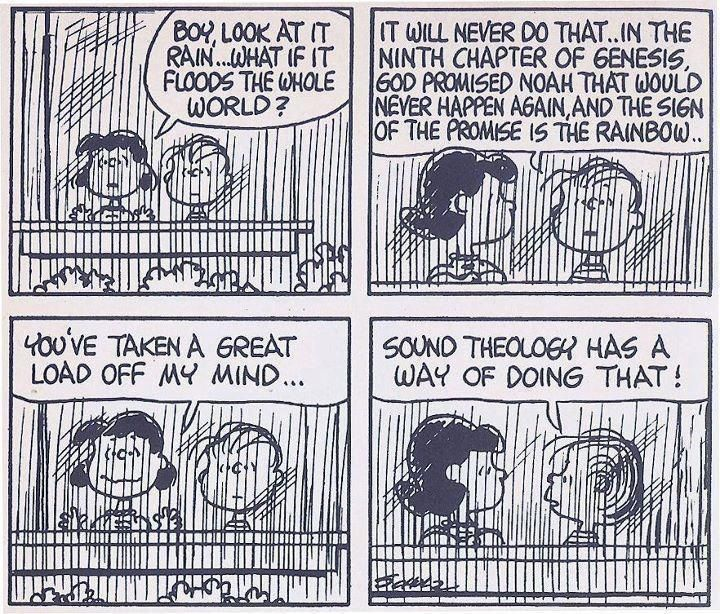
\includegraphics[height=\paperheight,width=\paperwidth]{./img/Peanuts-2Bsnoopy-2Band-2Bsound-2Btheology-2Bflood.jpg}}
    \setbeamertemplate{navigation symbols}{}
    \begin{frame}[plain]
    \end{frame}
    }


\begin{frame}[label=sec-1-2]{Modern era}
Given an understanding of the modern period beginning with the Reformation:
\begin{itemize}[<+->]
\item What characteristics are associated with the period?
\item What might characterize a ``post-modern'' period?
\end{itemize}
\end{frame}

\begin{frame}[label=sec-1-3]{History}
What does the following quote mean:

\begin{quote}
All histories, including the history of Christian theology, rest on the interplay between remembering and forgetting.'' (xxiv)
\end{quote}
\end{frame}

\begin{frame}[label=sec-1-4]{Denominational History}
The limits to our perspective (on things) is sometimes vast:
\begin{itemize}[<+->]
\item most of us learn church theology and church history from a denominational perspective
\item we enter the study through a particular portal
\item understanding will come through self-awareness of our own limitations
\end{itemize}
\end{frame}

\begin{frame}[label=sec-1-5]{Limitations and warnings (p. 2)}
Placher sets parameters for his text:
\begin{enumerate}[<+->]
\item It is history of Christian theology, not general history, intellectual history, etc.
\item Theology means the systematic reflection on one's faith. (experience?) An ``elite'' enterprise?
\item Much ends up being ignored
\item Too favorable picture of ``theology''?
\end{enumerate}
\end{frame}

\section{Introductory issues}
\label{sec-2}
\begin{frame}[label=sec-2-1]{Biblical interpretation}
\begin{itemize}
\item But it has changed over the centuries
\item Why would the 5th c. bishop respond so (xvii)
\item Need to believe what biblical authors believed? (xvii)
\item Rom 1 on homosexuality (xvii)
\end{itemize}
\end{frame}

\begin{frame}[label=sec-2-2]{vocabulary}
\begin{itemize}
\item Postliberal (xiv)
\item doctrine: set of beliefs, creed, etc.
\item Christology (xxi) \ldots{} place of suffering, identification with God
\item analytic philosophy:
\item meaning of faith and history
\item fundamentalism
\item positivism (xvi)
\item transcendence (xviii) immanence (xx)
\item scientific worldview (xix)
\end{itemize}
\end{frame}

\begin{frame}[label=sec-2-3]{names of theologians}
\begin{itemize}
\item Karl Barth
\item Paul Tillich
\item Rudolf Bultmann (xvi)
\item John Calvin
\item Isaac Newton
\item Galileo
\end{itemize}
\end{frame}
\begin{frame}[label=sec-2-4]{How talk about God (before and after modernity)}
\begin{itemize}[<+->]
\item ``Thing signified'' vs. ``means of signifying'' (xx)
\item analogical
\item univocal vs. equivocal
\end{itemize}
\end{frame}
\section{Groupwork}
\label{sec-3}
\begin{frame}[label=sec-3-1]{Some basic themes}
\begin{enumerate}
\item Humanity and Divinity of Christ
\item Reason and revelation
\item Works and Grace
\item Spirit and Structure
\item Church and State
\end{enumerate}
\end{frame}
% Emacs 24.3.1 (Org mode 8.2.3c)
\end{document}
